\documentclass[aspectratio=169, ignorenonframetext]{beamer}
\usepackage{pgf}

\mode<article>{
  \usepackage{fullpage}

}

\mode<presentation>
{
%   \usetheme{Madrid}
%   \useinnertheme{circles}
  \setbeamertemplate{navigation symbols}{}
%   \usetheme[hideothersubsections, width=2.4cm]{Hannover}
%   \usetheme{Antibes}
%   \usetheme{Montpellier}
%   \usetheme{Singapore}
  \usetheme{Darmstadt}
%   \usecolortheme{seahorse}
%   \usecolortheme{orchid}
  \setbeamertemplate{footline}
  {%
%     \begin{beamercolorbox}{section in head/foot}
%       \usebeamercolor{bg}
       \hskip 1em \footnotesize \insertframenumber{} / \inserttotalframenumber%\hskip 41em \includegraphics[height = .5cm]{../../../../bilder/cc_by-nc_eu.png}
% % cc_by-nc_eu.png: 403x141 px, 72dpi, 14.22x4.97 cm, bb=0 0 403 141
%
% % bwslogo_3.png: 476x392 px, 300dpi, 4.03x3.32 cm, bb=0 0 114 94
%
%       %\hskip 5em
%       %       \input{../bilder/cc_by.png}
%       %\includegraphics[height=.5cm]{../../../../bilder/bwslogo_3.png}
%     \end{beamercolorbox}%
  }
  \usepackage{beamerfoils}
}
\usepackage[german]{babel}
\usepackage[utf8]{inputenc}
\usepackage{times}
\usepackage[T1]{fontenc}
\usepackage{pgf}
\usepackage{pgfpages}
\usepackage{eurosym}
\usepackage{graphicx}
\usepackage{amsmath}
\usepackage[siunitx,european]{circuitikz}
\usepackage{ulem}
\usepackage{listings}
\usepackage{svg}
%
\lstset{numbers=left, numberstyle=\tiny, stepnumber=2, numbersep=5pt, language = C++, alsolanguage=XML}
% \MyLogo{\includegraphics[height=1cm]{../../../../bilder/bwslogo_3.png}}
% % \includegraphics{../../bilder/bwslogo_3.png}
% % bwslogo_3.png: 476x392 px, 300dpi, 4.03x3.32 cm, bb=
%
\only<article>{
  \usepackage[colorlinks=true,linkcolor=blue,filecolor=magenta,urlcolor=cyan]{hyperref}
}

\only<presentation>{
  \usepackage{hyperref}
}


\title{Arbeitsunterlagen zu FOS Elektrotechnik, technische Informatik, Mechatronik Themenfeld 12.1}
\subtitle{Gleichstromnetzanalyse - Teil 1}
\date{V 0.5.1 \\ Stand: \today}%\\

\institute[BWS Hofheim]{Brühlwiesenschule, Hofheim}
\author{Thomas Maul}

\titlegraphic{Für eigene Teile gilt: 
\includegraphics[height=1cm]{cc_by-nc_eu.png}}

\begin{document}
  \only<article>{
    \maketitle
    \tableofcontents
    \clearpage
  }
  \begin{frame}<beamer>
    \titlepage
    % \hyperlink{Teil_2}{\beamerbutton{Go part 2}}
  \end{frame}
  % \AtBeginSection[] % Do nothing for \section*
  % {
  %   \begin{frame}<beamer>
  %     \frametitle{Inhalt}
  %     \tableofcontents[currentsection]
  %   \end{frame}
  % }
% \begin{frame}{Was bisher geschah}
%     \begin{itemize}
%         \item Atome und Elektronen
%         \item Ladungen im Sinne der Elektrotechnik
%         \item Gleichstrom und Wechselstrom
%         \item Widerstand, Strom, Spannung, Leistung
%     \end{itemize}
% \end{frame}


% \part{Themenfeld 12.1 - Gleichstromnetzanalyse}
\begin{frame}
  \partpage
  %   \tableofcontents[hidesubsections]
\end{frame}
\begin{frame}<beamer>
  \frametitle{Inhalt}
  \begin{columns}
    \column{.5\textwidth}
    \tableofcontents[sections={1-4},hidesubsections]%currentsection]
    ZAP = In der Themenliste der Abschlussprüfung genannt.
    \column{.5\textwidth}
    \tableofcontents[sections={5-},hidesubsections]%currentsection]
  \end{columns}
\end{frame}
\section[KnotenV]{Knotenspannungsverfahren (ZAP)}
\begin{frame}{Knotenspannungsverfahren (Teil 1)}
  \subtitle{alternative Benennung: Knotenpotentialverfahren}
  \begin{itemize}
    \item Ein Knoten wird Bezug (z. B. Masse)
    \item Alle Widerstände in Leitwerte umwandeln ($G = \frac{1}{R}$)
    \item Spannungsquellen in Stromquellen umwandeln
    \item Knoten durchnummerieren ($\varphi_1 .. \varphi_n$)
    \item Gleichungen aufstellen
  \end{itemize}
\end{frame}

\begin{frame}{Knotenspannungsverfahren (Teil 2)}
  \begin{columns}
    \begin{column}{.65\textwidth}
      \begin{itemize}
   \item Hauptdiagonale: Alle Leitwerte am Knoten (pos. Vorzeichen)
   \item Nebendiagonalen: Alle Verbindungen zwischen Knoten i (Zeile) und j (Spalte) wichtig: neg. Vorzeichen
  \end{itemize}
  \begin{align}
   \left(
   \begin{array}{ccc|c}
     G1+G3+G5 & -G3 & -G5 & I_{q1}\\
     -G3 & G2+G3+G6 & -G6 & 0\\
     -G5 & -G6 & G4+G5+G6 & 0
   \end{array}
   \right)
  \end{align}
   \end{column}
   \begin{column}{.3\textwidth}
    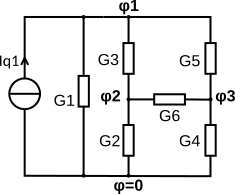
\includegraphics[scale=.7]{messbruecke3_1.png}
   \end{column}
  \end{columns}
\end{frame}

\begin{frame}{Knotenspannungsverfahren (Teil 3)}
   \begin{align}
   \left(
   \begin{array}{ccc}
     G1+G3+G5 & -G3 & -G5 \\
     -G3 & G2+G3+G6 & -G6 \\
     -G5 & -G6 & G4+G5+G6
   \end{array}
   \right)
   \cdot
    \left(
   \begin{array}{c}
    \varphi_1\\
    \varphi_2\\
    \varphi_3
   \end{array}
    \right)
   =
   \left(
   \begin{array}{c}
    I_{q1}\\
    0\\
    0
   \end{array}
    \right)
  \end{align}

  $\varphi_n$ = Spannungen der Knoten zum Bezugsknoten hier $\varphi = 0$
\end{frame}
\end{document}
